\documentclass[tikz,margin=1cm]{standalone}

\usepackage{pgfplots}
\pgfplotsset{compat=1.16}

\begin{document}
        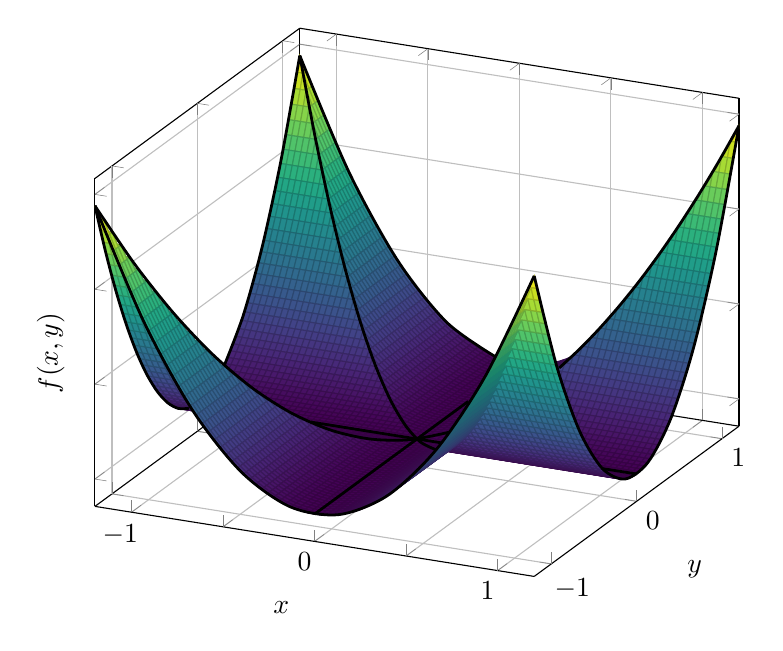
\begin{tikzpicture}
            \begin{axis}[
                colormap name=viridis,
                % 3d box,
                width=10cm,
                view={25}{20},
                axis equal image,
                % enlargelimits=false,
                grid=major,
                domain=-1.2:1.2,
                samples=75,
                yticklabels={,$-1$,$0$,$1$},
                xticklabels={,$-1$,,$0$,,$1$},
                zticklabels={,,},
                xlabel=$x$,
                ylabel=$y$,
                zlabel={$f(x, y)$},
                ]
                \addplot3 [y domain = -1.2:1.2, surf]
                {(x*x+y*y-abs(x*x-y*y))/2};
                \addplot3[domain=-0.19:1.2, samples=10, smooth, samples y =0, line width=1pt] ({-x}, {x}, {x^2});
                \addplot3[domain=0.53:1.2, samples=10, smooth, samples y =0, line width=1pt] ({x}, {x}, {x^2});
                \addplot3[domain=-1.2:0.12, samples=10, smooth, samples y =0, line width=1pt] ({x}, {x}, {x^2});
                \addplot3[domain=-0.58:0.13, samples=2, smooth, samples y =0, line width=1pt] ({x}, 0, 0);
                \addplot3[domain=1.01:1.2, samples=2, smooth, samples y =0, line width=1pt] ({x}, 0, 0);
                \addplot3[domain=-1.2:0.6, samples=2, smooth, samples y =0, line width=1pt] (0, {x}, 0);
                \addplot3[domain=-1.2:1.2, samples=10, smooth, samples y =0, line width=1pt] ({x}, -1.2, {x^2});
                \addplot3[domain=-1.2:1.2, samples=10, smooth, samples y =0, line width=1pt] (1.2, {x}, {x^2});
                \addplot3[domain=-1.2:-0.1, samples=10, smooth, samples y =0, line width=1pt] (-1.2, {x}, {x^2});
                \addplot3[domain=0.32:1.2, samples=5, smooth, samples y =0, line width=1pt] (-1.2, {x}, {x^2});
                \addplot3[domain=-1.2:-0.13, samples=5, smooth, samples y =0, line width=1pt] ({x}, 1.2, {x^2});
            \end{axis}
        \end{tikzpicture}
\end{document}
